% !TeX spellcheck = en_GB

\todo{general introductory sentence about network mon}

\section{Intrusion Detection Systems (IDS)}
\label{sec:background:network:ids}

\begin{comment}
		\begin{itemize}
		\item \enquote{A good network intrusion detection system (IDS) can have an enormous positive impact on the overall security of your oragnization} \parencite{Northcutt2005}
		\item \enquote{By detecting malicious activity, network intrusion detection enables you to identify and react to threats against your environment, as well as threasts that your hosts might be directing at hosts on other networks.} \parencite[p. 201]{Northcutt2005}
		\item \enquote{Without intrusion detection, you may never know about an attack that doesn't damage your host, but simply extracts information[...]. Without intrusion detection, you will be unaware of these events until it's much too late.} \parencite[p. 202]{Northcutt2005}
		\item Not only identifies attacks, but also reveals attack attempts and probing \parencite[p. 202]{Northcutt2005}
		\item 
	\end{itemize}
\end{comment}

Good network security consists of many parts, covering a huge variety of methods and functions. \hint{This sounds weird and artificial.}
As one of these parts \enquote{a good \gls{ids} can have an enormous positive impact on the overall security [...]}. \parencite{Northcutt2005}
The basic idea is to monitor the network traffic passing by sensors and therefore be able to detect malicious activities.
This allows the \gls{ids} to detect and identify threasts against the own environment or theats ones own hosts impose to other environments, due to an infection with malware.
Without intrusion detection one might never detect attacks, that do not influence normal operations but for instance extract information.

Further, \gls{ids} may also identify attack attempts and probing, allowing to further harder the environment and take precautions.

Nowadays \glspl{ids} are a commonly deployed in \gls{ip} networks. There are different kinds of \glspl{ids}, which can be discriminated by working principle. The following section is giving an overview of the most common technologies. \parencite[cf.][pp.~201-202]{Northcutt2005}

\subsection{Signature-based Intrusion Detection Systems (SIDS)}
\label{sec:background:network:ids:sig}

\begin{comment}
	\begin{itemize}
		\item \enquote{[...] IDS signature is a pattern you are looking for in traffic.} \parencite{Northcutt2005}
		\item \enquote{When a signature for an attack matches observed traffic, an alert is generated, or the event is otherwise recorded.} \parencite{Northcutt2005}
		\item \enquote{Many signatures are protocol or application specific;} \parencite{Northcutt2005}
		\item requires to update a curated set of signatures regularly \parencite{Northcutt2005}
		\item \enquote{Signature development is always a balancing act. A specific signature might be extremely accurate in identifying a particular attack [...] [but] If an attacker slightly modifies the attack, the signature might not be able to identify it at all.} \parencite{Northcutt2005}
			\subitem precision/recall balance
		\item \enquote{Every intrusion detection system generates false positives.} \parencite[p.~205]{Northcutt2005}
		\item \enquote{By selecting a solid IDS product and tuning your sensors, you can reduce false positives, but you can't completely eliminate them.} \parencite[p.~205]{Northcutt2005}
		\item \enquote{[...], but each false negative is a legitimate attack or incident that IDS failed to notice.} \parencite[p.~206]{Northcutt2005}
		\item \enquote{Besides false positives, you might also have alerts that address legitimate problems that you simply don't care about.} (Unwanted Alerts) \parencite[p.~206]{Northcutt2005}
		\item 
	\end{itemize} 
\end{comment}

One of the more traditional \gls{ids} principles are signature based systems.
They work by comparing patterns (signatures) of malicious traffic to the observed traffic. When a pattern matches an alert is raised.
This requires many protocol and application specific signatures, which are difficult to create and maintain, since a good balance between being too generic and being too specific needs to be found.

A signature which is too generic, may cause many false positives. This might lead to an elimination of any positive effect of the \gls{ids}, since real alerts become impossible to spot among the false positives.
In contrast, however, a signature which is too specific might suffer from a too narrow scope. Meaning, that it might be really precise in classifying one particular attack, but fails to do so if an attacker just slightly modifies it.

As a result, a valuable \gls{ids} solution is characterised by an balanced precision/recall ratio. This can be archived by using a good signature database and fine tuning the sensors.
However, it is to note, that every \gls{ids} will produce false positives. This derives out of the consideration, that each false negative is an legitimate attack, which was not detected. Therefore a slight tendency to (over) sensitivity is sensible.

Other than false positives, there might be legitimate alerts that are of no interest. These unwanted alerts should be blocked, to not numb \alert{(is this the right word here?)} the system administrator. \parencite[cf.][pp.~205-206]{Northcutt2005}
	
\subsection{Anomaly-based Intrusion Detection Systems (ABIDS)}
\label{sec:background:network:ids:anomaly}
	
\begin{comment}
	\begin{itemize}
		\item \enquote{establishing baselines of normal network activity over a period of time, then detecting significant deviations from the baseline.} \parencite[p. 203]{Northcutt2005}
		\item \enquote{[...] later, if the IDS sensor sees a high volume of traffic involving a previously unused service on a host, this could indicate a distributed denial of service (DDoS) attack against the host or a compromised host providing a new service.} \parencite{Northcutt2005}
		\item \enquote{[...] drawback of this type of anomaly detection is that the baseline needs to be updated constantly to reflect authorized changes[...]} \parencite{Northcutt2005}
		\item \enquote{If the baseline can be kept current, or if the environment is quite static and the baseline changes rarely, anomaly detection can be extremely effective at identifying certain types of attacks [...]} \parencite{Northcutt2005}
		\item \textbf{\enquote{Unfortunately, this type of anomaly detection cannot identify most other types of attacks, so it is best used to complement other IDS technologies.}} \parencite{Northcutt2005}
		\item \enquote{[...] can [...] identifying certain previously unknown instances of attacks [...]} \parencite{Northcutt2005}
		\item \enquote{cannot determine the intent of an attack} \parencite{Northcutt2005}
	\end{itemize}
\end{comment}

Another major technology used in \glspl{ids} is anomaly detection. (cf. Section~\ref{sec:background:network:novelty})
Unlike signature based methods (cf. Section~\ref{sec:background:network:ids:sig}) it does not require an predefined set of rules, rather deploying anomaly detection it is able to auto-generate rules specific for the monitored network and then perform whitelisting using these rules.

This is archived by having a so called training phase before deploying the \gls{ids}. During the training phase a baseline model is established using the normal network activity over period of time. It is to note, that this period should be long enough to cover normally recurring usage cycles, e.g. day-time/night-time, weekday/weekends, etc.

After an successful training phase the \gls{ids} uses the generated baseline model to compare bypassing traffic against it.
If it detects a significant deviation from it, an alert is raise as it indicates unusual network activities.
For instance, if an internal host in an \gls{ip} network, produces suddenly a lot of outbound traffic, which was not the case before, it might indicate an infection on this host.

This example illustrates 2 primary drawbacks of purely anomaly-based \glspl{ids}: 
First, the system can not identify which kind of attack it detects, it merely identifies an anomaly. To identify the intention of the attack it would need to be combined with a rule system or signature-based approach.

Second, the increased outbound traffic in the example could have been generated by a new legitimate software, i.e. a website crawler.
Consequently, strictly separated training and operational phases lead to poor adaption of the \gls{ids} to a changing environment.
This could be mitigated by updating the baseline model during normal operation, so t accommodates for changes.
However, by continuing the training phase, attacker might be able to reprogram the baseline in their favour by injecting malicious packets very rarely at the beginning, but then increase the amount steadily.
By doing so the relative deviation from the continuing trained baseline model stays relatively low and will therefore not trigger an alert.
This means, the decision if the baseline model should be trained continuously has to be made under careful consideration of the nature of the network to be monitored.

All in all, anomaly-based \glspl{ids} are ideal to identify prior unknown threats and attacks in relatively stable environments. However, it might also identify (legitimate) changes in the environment as anomaly. Additionally it might be unable to detect attacks which mimic regular behaviour and only deviate slightly from legitimate traffic.
As a result, anomaly-based \glspl{ids} should be combined with other \gls{ids} technologies, when used to protect production systems.
\parencite[cf.][pp.~203-204]{Northcutt2005} \todo{check pages}
	
	\subsection{State-based Intrusion Detection Systems\hint{??}}
	\label{sec:background:network:ids:state}
	
	\begin{itemize}
		\item cf. \textcite{Whitman2009} page 306 
	\end{itemize}

% ------------------------------------------------------------------------------
\section{Flow Monitoring}
\label{sec:background:network:netflow}

\begin{comment}
	\begin{itemize}
		\item active
			\begin{itemize}
				\item inject additional traffic to measure things \parencite{Hofstede2014}
				\item e.g. ping, traceroute
			\end{itemize}
		\item passive
			\begin{itemize}
				\item "observe existing traffic as it passes by" \parencite{Hofstede2014}
				\item e.g. packet capture "This method generally provides most insight into the network traffic, as complete packets can be captured and further analyzed. However, in high-speed networks with line rates of up to 100 Gbps, packet capture requires expensive hardware and substantial infrastructure for storage and analysis." \parencite{Hofstede2014}
				\item "Another passive network monitoring approach that is more scalable for use in high-speed networks is flow export, in which packets are aggregated into flows and exported for storage and analysis." \parencite{Hofstede2014}
				\item  "a set of IP packets passing an observation point in the network during a certain time interval, such that all packets belonging to a particular flow have a set of common properties." \parencite{Claise2013}
				
			\end{itemize}
	\end{itemize}
\end{comment}

Following the idea of network monitoring with \glspl{ids}, multiple method are being used. They can be roughly classified into active and passive. 
Active approaches work by injecting additional traffic into the network to obtain certain measurements, like ping or traceroute.
Passive techniques, on the contrary, only observe existing traffic passing by a measurement point and derive measurements from it. The most simple and straight forward passive approach would be packet capturing. Also it provides the most insights into bypassing traffic, since in-depth analysis are possible. However, a full packet capture raises problem within high-speed networks or if network bandwidth is highly limited, like it is in field bus networks. This is especially problematic if information are required to be analysed by an central authority to obtain world-view. The problems arising here include high storage consumption, excessive infrastructure requirements, and unnecessary high utilisation of network bandwidth. \todo{relevant in already highly utilised networks, etc.}
\parencite[cf.][]{Hofstede2014}
Especially the additional high network utilisation is of notable concern in field bus networks used in \glspl{bas}. Effectively doubling the traffic in the sub-lines, as well as routing the monitoring traffic to central place would not only occupy a good portion of free bus capacity, but would also render network separation (cf. Section~\ref{sec:background:bas:knx:security}) useless. Consequently, soften the security in the network and possibly decreasing the responsiveness of commands dramatically.

A another predominantly used passive approach is flow monitoring, which focusses on analysing flows within a network rather than analysing a full packet dump. Therefore archiving a significant data reduction and consequently requiring only a fraction of the bandwidth, while also keeping principles like network separation in tact, since only aggregated statistical data is transferred.
A flow is defined by \textcite{Claise2013} as \enquote{a set of IP packets passing an observation point in the network during a certain time interval, such that all packets belonging to a particular flow have a set of common properties.}
Mentioned common properties most commonly include various header fields, like port, source- and destination address, but also the used application layer protocol or metadata derived from the packet content.
It is widely used for \enquote{security analysis, capacity planning, accounting, and profiling, among others.} \parencite{Hofstede2014}
Common protocols used for flow monitoring are \gls{netflow} \parencite{Claise2004} and \gls{ipfix} \parencite{Claise2013}.

\todo{not predominantly used for security, but network congestion avoidance/mitigate.}

\begin{figure}
	\centering
	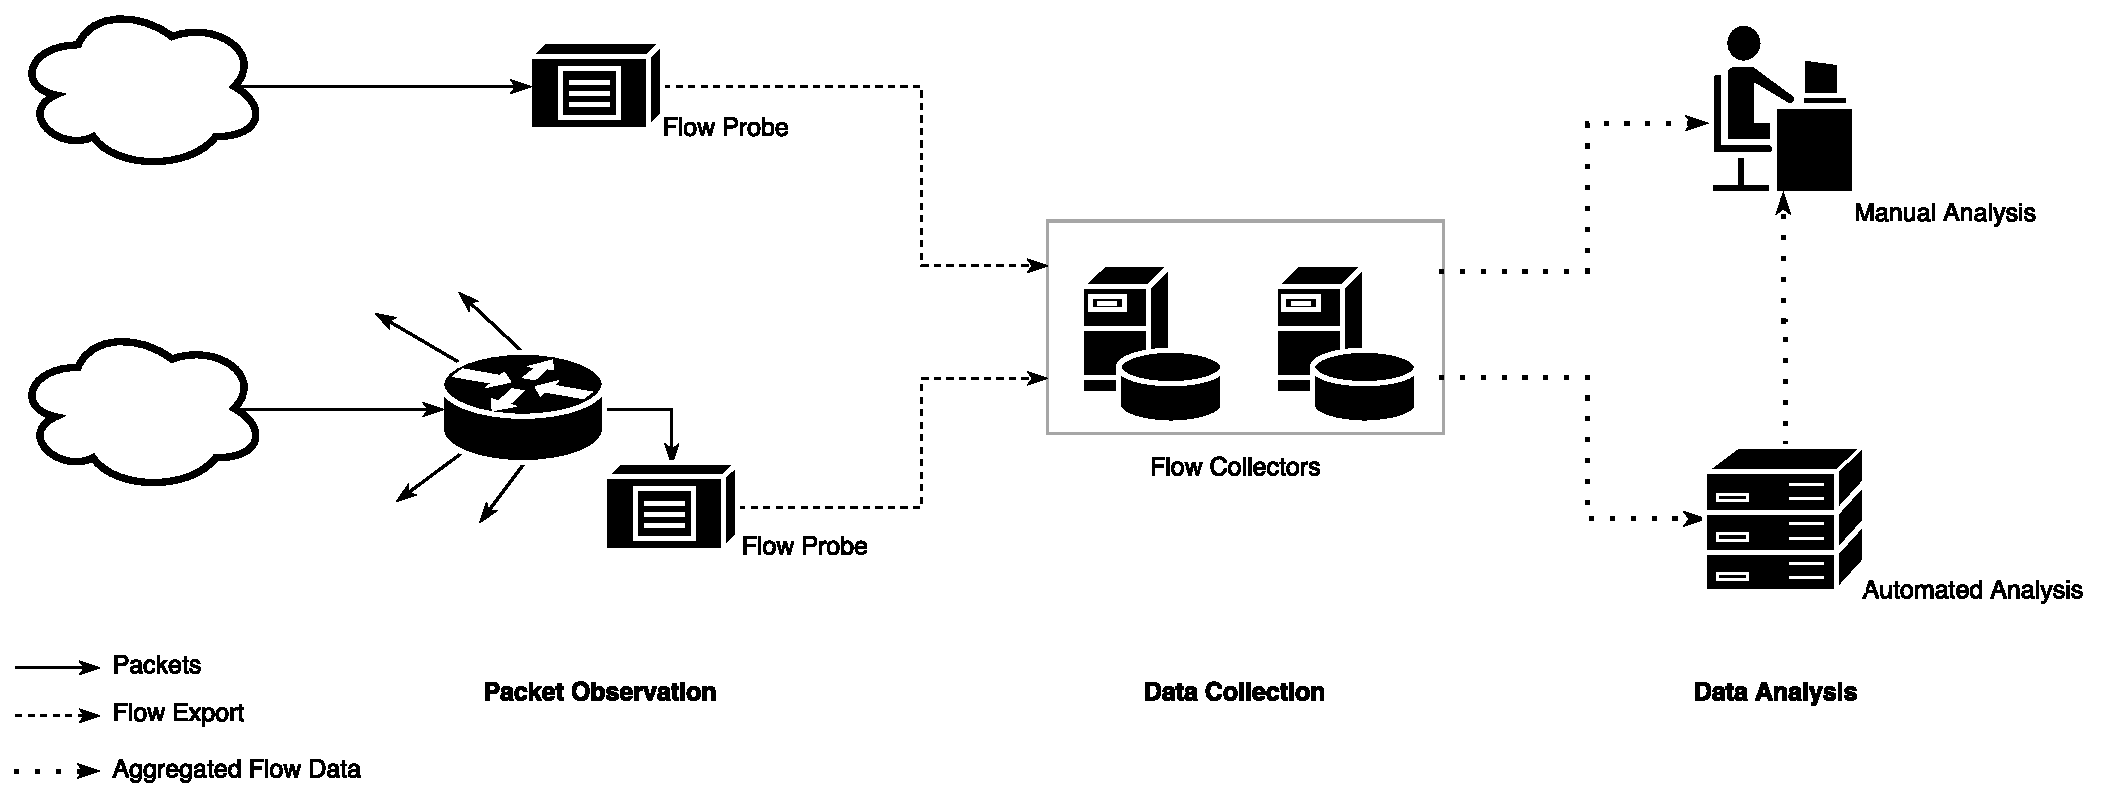
\includegraphics[width=\textwidth]{figures/200-netflow-architecture.pdf}
	\caption[Simplified flow monitoring system architecture]{Simplified flow monitoring system architecture. \parencite[cf.][]{Hofstede2014} \todo{adjust font size}}
	\label{fig:background:network:netflow:architecture}
\end{figure}

Typical flow monitoring architectures can be roughly separated into 3 stages. (cf. Figure~\ref{fig:background:network:netflow:architecture})
The first one, being Packet Observation and Flow Export, will observe bypassing traffic. Further the observed traffic is aggregated into flows, using common properties as selectors. (cf. above\alert{???}) After a flow is terminated, either by closing the underlying connection or by timeout, a record of it is exported and send of to the Flow Collector.
This stage could be implemented by a stand-alone device or within an appliance like a router with flow export capability. \parencite[cf.][]{Hofstede2014}

The exported flow are then receive by the Data Collector, which main task are storage and processing.
Exported flows contain \enquote{information about a specific flow that was observed at an observation point} \parencite{Claise2013}, which may include characteristic properties like \gls{ip} addresses and port number, as well as measured properties like packet count or overall flow size in bytes. \parencite[cf.][]{Hofstede2014}
In scope of \glspl{bas}, like \gls{knx}, characteristic properties could include source and destination address, and \gls{apci}. Hop count, payload length, and \gls{tpci} would then be used as measured properties.

Finally the last stage is concerned with the data analysis. This can be done in a manual, exploratory way, which is often the case in research projects. In more production oriented setups the analysis is often automated and integrated into the Data Collector.
The data analysis commonly includes functions like traffic profiling, correlation, anomaly and intrusion detection (cf. Section~\ref{sec:background:network:ids}), and classification and characterisation. \parencite[cf.][]{Hofstede2014}
In this work mainly anomaly and intrusion detection is of interest.

% ------------------------------------------------------------------------------
\section{Anomaly, Outlier, and Novelty Detection}
\label{sec:background:network:novelty}

The analysis of flows or general network traffic as describes in Section~\ref{sec:background:network:ids:anomaly}~and referenced in Section~\ref{sec:background:network:netflow}, relies on algorithm and techniques to detect data points which deviate from the normal expected behaviour. These algorithms and techniques can be found \alert{(better phrasing)} under the term Anomaly, Outlier, or Novelty Detection.
The aim of this section is to provide a classification of these algorithms with benefits and drawbacks.
Further, an overview of the working principle is provided for a small selection of them.

% ------------------------------------------------------------------------------
\subsection{Classification of Anomaly, Outlier, and Novelty Detection Approaches}
\label{sec:background:network:novelty:class}

\begin{comment}
	\begin{itemize}
		\item cf. \textcite{Hodge2004}
		\item Type 1: "Determine the outliers with no prior knowledge of the data" \parencite{Hodge2004}
			\subitem "unsupervised clustering" \parencite{Hodge2004}
			\subitem "assumes that errors or faults are separated from the ‘normal’ data and will thus appear as outliers" \parencite{Hodge2004}
			\subitem " predominantly retrospective and is analogous to a batch-processing system" \parencite{Hodge2004} - Requires a bunch of data to begin with
			\subitem " requires that all data be available before processing" \parencite{Hodge2004}
			\subitem "data is static" \parencite{Hodge2004}
			\subitem "two sub-techniques" \parencite{Hodge2004}
			\subitem -> "outlier diagnostic approach highlights the potential outlying points" \parencite{Hodge2004} and "prune the outliers and fit their system model to the remaining data until no more outliers are detected" \parencite{Hodge2004}
			\subitem -> "accommodation that incorporates the outliers into the distribution model generated and employs a robust classification method" \parencite{Hodge2004} which "can withstand outliers in the data and generally induce a boundary of normality around the majority of the data" \parencite{Hodge2004}
			\subitem "Non-robust methods are best suited when there are only a few outliers in the data set" \parencite{Hodge2004}
			\subitem "a robust method must be used if there are a large number of outliers to prevent this distortion" \parencite{Hodge2004}
		\item Type 2: "Model both normality and abnormality." \parencite{Hodge2004}
			\subitem "supervised classification" \parencite{Hodge2004}
			\subitem "requires pre-labelled data" \parencite{Hodge2004}
			\subitem "The entire area outside the normal class represents the outlier class" \parencite{Hodge2004}
			\subitem "best suited to static data" \parencite{Hodge2004} "classification needs to be rebuilt from first principles if the data distribution shifts" \parencite{Hodge2004}
			\subitem "can be used for on-line classification" \parencite{Hodge2004} learning while new samples are classified
			\subitem "require a good spread of both normal and abnormal data" \parencite{Hodge2004}
			\subitem "classification is limited to a ‘known’ distribution" \parencite{Hodge2004}
			\subitem "cannot always handle outliers from unexpected regions" \parencite{Hodge2004}
		\item Type 3: "Model only normality [...]" \parencite{Hodge2004}
			\subitem "novelty detection" \parencite{Hodge2004} " semi-supervised recognition or detection task" \parencite{Hodge2004}
			\subitem "needs pre-classified data but only learns data marked normal" \parencite{Hodge2004}
			\subitem "suitable for static or dynamic data" \parencite{Hodge2004}
			\subitem "can learn the model incrementally as new data arrives" \parencite{Hodge2004}
			\subitem "aims to define a boundary of normality" \parencite{Hodge2004}
			\subitem "requires the full gamut of normality to be available for training to permit generalisation" \parencite{Hodge2004} but "requires no abnormal data" \parencite{Hodge2004}
			\subitem this is good, because "Abnormal data is often difficult to obtain or expensive in many fault detection domains [...]" \parencite{Hodge2004}
			\subitem "as long as the new fraud lies outside the boundary of normality then the system will be correctly detect the fraud" \parencite{Hodge2004}
	\end{itemize}
\end{comment}

Anomaly, Outlier, or Novelty Detection describes a class of algorithms to detect data points which deviate from the expected normal behaviour.
Or as defined by \textcite{Grubbs1969}, \enquote{an outlying observation, or outlier, is one that appears to deviate markedly from other members of the sample in which it occurs.}
In the following this definition will be used as an understanding for outliers, which is exchangeable for anomaly or novelty. \alert{(think about this!)}

The general class of algorithms for Anomaly, Outlier, and Novelty Detection can be divided into 3 sub-classes, based on which kind of data the algorithms require to be trained\alert{~and executed}.
The first sub-class describes algorithms, which are able detect outliers without prior knowledge of the data, also known as unsupervised clustering.
This means, the data points in a training set are not require to be labelled as \emph{normal} or \emph{outlier}, which is archived by relying on the assumption, that non-normal data is separated from normal data, thus appearing as outlier.
Accordingly, a substantial amount of data is required to begin with, since these kind of algorithms word \enquote{predominantly retrospective} \parencite{Hodge2004}.
Thus requiring (all) data to be available before processing and assuming it to be static.
Within this technique, 2 approaches  are used for training the model. 
The first identifies potential outliers and then continues to prune them from the original data set and fit the model to the remaining data points. This is iterated until no more outliers are detected. This non-robust method is well suited when only a few outliers are in the data set.
The second approach, however, accommodates the outliers into the distribution model and then applies a robust classification method. This is a better suited for data sets with higher numbers of outliers, since a robust classification method can withstand outliers in the data set by inducing boundaries of normality around large portions of the data. \parencite[cf.][]{Hodge2004}

The second sub-class within Outlier Detection techniques works by modelling both, normality and outliers, it is also known as supervised classification.
Therefore it requires pre-labelled data in the training phase, labelled as \emph{normal} or \emph{outlier}. Since both are used to build the model, a good spread of \emph{normal} and \emph{outlying} data is required, which also limits the classification to the known distribution of such.
As a result the whole classification model needs to be rebuild from ground up, as soon as the distribution shifts.
However, a major benefit of this method is, that it is allows for training the model while new data points are being classified, which is also known as on-line classification. \parencite[cf.][]{Hodge2004}

The third and last sub-class in Outlier Detection techniques models only normality. These techniques are often described as novelty detection or semi-supervised recognition.
It requires also pre-labelled data, but compared to the second type it only works with \emph{normal} labelled data points. Consequently the full gamut of normality is required to train an precise model. On the other hand no \emph{outlying} data points are required for training, which is highly beneficial in certain, data-sparse, scenarios, when abnormal data is difficult to obtain.
However, the training data must not contain outliers, otherwise they will be assumed to be a part of normality.
Generally the aim of this approach is to establish a tight boundary around normality and is therefore suitable for static as well as dynamic data.
If a new data point lies outside of the this boundary it is considered an \emph{outlier}, if not it is part of the \emph{normal} data.

% ------------------------------------------------------------------------------
\subsection{k-Nearest Neighbour}
\label{sec:background:network:novelty:knn}

\begin{comment}
	\begin{itemize}
		\item \enquote{Given a collection of data points and a query point in an m-dimensional metric space, find the data point that is closest to the query point.} \parencite{Beyer1999}
		\item \enquote{determines whether or not a point lies in a sparse region of the feature space by computing the sum of the distances to the k-nearest neighbours of the point} \parencite{Eskin2002}
		\item \enquote{[...] points in dense regions will have many points near them and will have a small k-NN score} \parencite{Eskin2002}
		\item \enquote{main problem [...] is that it is computationally expensive to compute the k-nearest neighbours of each point} \parencite{Eskin2002}
	\end{itemize}
\end{comment}

Among the techniques which can be used for clustering and hence for anomaly detection \gls{knn} is one of more established one, initially published by \textcite{Fix1951}.
The problem is described, that for any given collection of data points in an m-dimensional metric feature space, to find the k nearest data points for an arbitrary query point. \parencite{Beyer1999}
It consequently uses the proximity of data points within the feature space, allowing \gls{knn} to work with unlabelled unclean data, making it a class 1 technique according to \textcite{Hodge2004}. (cf. Section~\ref{sec:background:network:ids:anomaly})

To determine if the query point is located in an sparse area, meaning it is an outlying observation, the sum of the distance to the k-nearest neighbours is calculated.
Data points with in denser area, representing normality, will have shorter distances to their neighbours. \parencite{Eskin2002}

\subsection{Local Outlier Factor}
\label{sec:background:network:novelty:lof}

\begin{comment}
	\begin{itemize}
		\item Proximity-based technique
		\item seems to be a good fit cf. \textcite{Lazarevic2003}
		\item works on unclean training data
		\item good selection of vectors and distance functions is required
		\item 11\% of the first 500 telegrams in \verb|eiblog.txt| are considered outliers
		\item density based
		\item base paper \textcite{Breunig2000}
		\begin{itemize}
			\item determines for each sample in the data-set its degree of \enquote{outlier-ness} \parencite{Breunig2000}
			\item definition outlier: \enquote{An outlier is an observation that deviates so much from other observations as to arouse suspicion that it was generated by a different mechanism.} \parencite{Hawkins1980}
			\item local approach
			\subitem therefore better than k-NN, because it accounts for different density of different cluster
			\subitem \enquote{most existing work in outlier detection lies in the field of statistics} \parencite{Breunig2000}
			\subitem counteracts different density of clusters \parencite{Breunig2000}
			\subitem outlier = point is further away from its nearest points than the other points are away from each other \parencite{Breunig2000}
		\end{itemize}
	\end{itemize}
\end{comment}

Another proximity based approach to outlier detection is the \glsfirst{lof}, introduced by \textcite{Breunig2000}. It is based on the \gls{knn} problem, but accounts for locality and is specifically designed for outlier detection.
With \gls{lof} an outlier is a data point which \emph{MinPts} nearest neighbours are further away then these neighbours from each other. 
Using this lemma, For each data point the degree of \enquote{outlier-ness}, or local outlier factor, is determined.

By not relying on a global threshold, the \gls{lof} can account for clusters of different density. Therefore, one could argue, that the \gls{lof} is not only proximity based, but rather density based. Further by not treating the classification of an outlying observation as a binary property, analysis made on top of the outlier classification can be more precise. \parencite[cf.][]{Breunig2000}

Moreover, the ability of \gls{lof} to work on unclean data and account for different density in clusters through locality, making it a good match for \gls{ids} solutions, as \textcite{Lazarevic2003} shows. Also \textcite{Zanero2004} conducted an experiment on using unsupervised learning algorithms for intrusion detection and found, that the problem of locality with \gls{knn} has to be addressed in order to be more precise in predictions, what \gls{lof} archives.

\subsection{Support Vector Machines}
\label{sec:background:network:novelty:svm}

\begin{comment}
	\begin{itemize}
		\item \enquote{The task of classification is to find a rule, which, based on external observations, assigns an object to one of several classes} \parencite{Muller2001}
		\item separate vector space by decision surfaces, setting boundaries between categories \parencite{Muller2001}
		\item \enquote{a learning algorithm for problems which are separable by hyperplanes} \parencite{Scholkopf2001a}
		\item \enquote{among all hyperplanes separating the data, there exists a unique optimal hyperplane, distinguished by the maximum margin of separation between any training point and the hyperplane} \parencite{Scholkopf2001a}
		
		\item One Class SVM
			\begin{itemize}
				\item aka. novelty detection
				\item all training data is considered good
				\item decision surface is fitted as close as possible to the training data
				\item new data outside this area, surrounded by decision surfaces, is considered an outlier
				\item \enquote{[...] does not require training data to be labelled to determine a decision surface.} \parencite{Lazarevic2003} (seems to be not exactly One-Class SVM)
				\item 
			\end{itemize}
	\end{itemize}
\end{comment}

Another technique to discriminate outliers from \emph{normality} is to precisely model \emph{normality}, as \textcite{Hodge2004} described as third class of outlier detection algorithms. (cf. Section~\ref{sec:background:network:novelty:class})
\glspl{svm} are a widely used technique in this field. Especially one-class \glspl{svm} are applied in outlier and intrusion detection. \parencite[cf.][]{Lazarevic2003,Eskin2002}
They classify data points by defining decision surfaces within the feature space, which separate categories. A learning algorithm fits these hyperplanes to prior labelled data, basically finding a rule to separate data points into different classes. 
In case of one-class \gls{svm}, which are predominantly used for outlier detection, there is only one category resembling \emph{normality}. Hence the training data must contain the full gamut of normal data points, without any contamination introduced by anomalies. \parencite[cf.][]{Muller2001,Scholkopf2001a}

As \textcite{Eskin2002,Lazarevic2003} showed, \gls{svm} are a good and viable techniques to be used in anomaly-based \glspl{ids}. However, since the way this model is trained requires for clean training data, it is increasingly hard to fit it into new networks and changing environments. (cf. Section~\ref{sec:background:network:ids:anomaly})
	
\subsection{Isolation Forest}
\label{sec:background:network:novelty:isoforest}
	
	\begin{itemize}
		\item \enquote{explicitly isolates anomalies rather than profiles normal instances} \parencite{Liu2008}
		\item \enquote{takes advantage of two anomalies’ quantitative properties} \parencite{Liu2008}
			\subitem \enquote{they are the minority}
			\subitem \enquote{have attribute-values that are very different}
	\end{itemize}

\subsection{Entropy based Outlier detection}
\label{sec:background:network:novelty:entropy}

The information entropy, introduced by \textcite{Shannon1948}, provides an effective way to determine the uncertainty of a given system or the information content of a variable. It is further also referred to as measurement for randomness. Especially later one is intuitively related to outlier detection.

\textcite{Toshniwal2014} are using these characteristics and propose an algorithm to cluster data streams and determine outliers. 
The basic principle is to try to fit every occurring data point to every existing cluster. The data point is then finally assigned to the cluster, where it produces the least increase of entropy. Finally, the relative change of entropy for assigning a data point to the nearest cluster (\emph{PCE}) is calculated. If this \emph{PCE} is higher than a prior defined threshold, the data point is considered an outlier.
However, this method requires access to all previous data points, which implies a high resource utilisation. To increase performance \textcite{Toshniwal2014} are only keeping a window of data in memory.
Further, it might be to consider to determine a kernel function, fitted to the individual dimensions. The entropy could then be calculated against the distribution function, rather than raw data.



\begin{comment}
\subsection{Elliptical Envelope}
\label{sec:background:network:novelty:envelope}
	
	\begin{itemize}
		\item tries to fit data to estimated \emph{shape}
		\item does not seem to be a good match, since it required to know the distribution of the vector fields
	\end{itemize}

\subsection{Statistical techniques}
\label{sec:background:network:novelty:stat}

\begin{itemize}
	\item "Some [...] are applicable only for single dimensional data sets" \parencite{Hodge2004}
	\item "requires no user parameters as all parameters are derived directly from data" \parencite{Hodge2004}
	\item e.g. "Grubbs’ method (extreme studentized deviate) (Grubbs, 1969) which calculates a Z value as the difference between the mean value for the attribute and the query value divided by the standard deviation for the attribute where the mean and standard deviation are calculated from all attribute values including the query value. The Z value for the query is compared with a 1\% or 5\% significance level" \parencite{Hodge2004} also cf. \textcite{Grubbs1969}
\end{itemize}

\subsection{Proximity-based techniques}
\label{sec:background:network:novelty:prox}

\begin{itemize}
	\item "no prior assumptions about the data distribution" \parencite{Hodge2004}
	\item "not feasible for high dimensionality data sets" \parencite{Hodge2004}
\end{itemize}	


%\subsection{Bayesian}
%\subsection{Pattern Matching}
\subsection{Autoassociative Kernel Regression (AAKR)}
	used by \textcite{Yang2006}
\end{comment}

%\section{Time-based Anomaly Detection}

\section{Methods of Feature Encoding}
\label{sec:background:network:features}

Most algorithms and techniques for Outlier Detection (cf. Section~\ref{sec:background:network:novelty}) work within a multi-dimensional vector space or feature space. Often it is not straight forward to map specific features of a data set into a vector space.
Problematic cases included when the possible expressions of a feature need to be model as equidistant to each other.
Alternatively, in certain cases it is necessary to reduce the amount of dimension a feature would add, because otherwise the resource utilisation would exceed sane boundaries.

\subsection{One-Hot encoding}
\label{sec:background:network:features:onehot}

Certain features in a dataset can represent markers or flags. In traditional data processing flags are often encoded as bit-field, where each bit represents one specific flag or marker, or as numerical value, where each number represents a state.
When using machine learning techniques, like Outlier Detection, directly on bit-fields or numerical encoded flags, a problem arises, especially with proximity base approaches.

For instance the \gls{apci} value encodes the application type in a \gls{knx} telegram as numerical value. (cf. Section~\ref{sec:background:bas:knx:communication})
For instance a \code{A\_GROUP\_VALUE\_WRITE} telegram is encoded with a value of \code{128}, whereby an \code{A\_GROUP\_VALUE\_READ} is encoded with a value of \code{000}, and \code{A\_INDIVIDUAL\_ADDRESS\_WRITE} with \code{192}.
The euclidean distance between those different \gls{apci} values would be 128, 64, and 0, which would indicate some kind of hierarchy or order.

However, for the sake of determining outliers, it is only of relevance if these values differ, the possibly induced hierarchy or order does not provide any information.
In other words the different expressions of this feature must be kept equidistant to each other.

To archive this, it is suggested in literature, to encode each expression as own dimension and only setting the expressed one to 1, leaving the rest at 0. This is referred to as \emph{one-hot} encoding. \parencite[cf.][]{Coates2011}

\subsection{Feature Hashing}
\label{sec:background:network:features:hashing}

When introducing multiple features in the vector space, the  amount of dimensions can increase rapidly, especially when using techniques like one-hot encoding (cf. Section~\ref{sec:background:network:features:onehot}).
This has huge implications with regards to resource consumption and more importantly to the feasibility of used algorithms on the vector space.
For instance proximity based approaches to Outlier Detection do not perform well in high dimensional vector spaces. \alert{cite needed}

To reduce the number of dimensions the amount of features could be reduced, or one could compress the feature vector. One method to archive compression by maintaining the informative value is called Feature Hashing or Kernel Trick. \parencite{Weinberger2009,Shi2009}
As the name suggests a specialised hash function is applied to the feature value to reduce the required dimensions down to a defined size.
This process is non reversible, which might have implications for further processing the results, e.g. using the coordinates of decision planes in \glspl{svm}.
Further, feature hashing introduces the possibility of hash collisions, especially when the targeted dimension number is low. Therefore the reduction needs to be considered carefully.
However, when compared to a random projection, to reduce dimensionality, the hashing-trick preserves the density and introduces no additional overhead. \parencite{Weinberger2009,Shi2009}

\subsection{Encoding Time}
\label{sec:background:network:features:time}



\begin{comment}
\begin{itemize}
	\item use feature direct as vector-dimension (not so good)
	\item OneHot encoding
		\subitem one vector-dimension per possible feature vector
		\subitem if feature has specific value, set dimension for this value to 1, the rest 0
		\subitem also cf. \textcite[][p. 12]{Eskin2002}, not mentioned as term, but good math-like description
		\subitem reversible
	\item Feature Hashing / Hashing Trick
		\subitem defined amount of dimensions
		\subitem feature value is hashed
		\subitem hash value is then used
		\subitem non reversible
		\subitem possibility of hash collision
		\subitem esp. when dimension count is low
		\subitem \enquote{\emph{hashing-trick:} one hashes high dimensional input vectors $x$ into a \emph{lower} dimensional feature space $\mathbb{R}^m$ with $\phi: X \rightarrow \mathbb{R}^m$} \parencite{Weinberger2009,Shi2009,Langford2007}
		\subitem \enquote{Different from random projections, the hashing-trick preserves sparsity and introduces no additional overhead to store projection matrices} \parencite{Weinberger2009}
	\item "normalize all [...] attributes to the number of standard deviations away from the mean." \parencite{Eskin2002}
		\subitem "scale based on the likelihood of the attribute values" \parencite{Eskin2002}
\end{itemize}
\end{comment}